\documentclass[10pt, oneside]{article} 
\usepackage{amsmath, amsthm, amssymb, calrsfs, wasysym, verbatim, bbm, color, graphics, graphicx, geometry}
\usepackage[most]{tcolorbox}
\usepackage{xcolor}
\usepackage{framed}
\colorlet{shadecolor}{blue!15}
\graphicspath{ {./} }

\geometry{tmargin=.75in, bmargin=.75in, lmargin=.75in, rmargin = .75in}  

\newcommand{\R}{\mathbb{R}}
\newcommand{\C}{\mathbb{C}}
\newcommand{\Z}{\mathbb{Z}}
\newcommand{\N}{\mathbb{N}}
\newcommand{\Q}{\mathbb{Q}}
\newcommand{\Cdot}{\boldsymbol{\cdot}}

\newtheorem{thm}{Theorem}
\newtheorem{defn}{Definition}
\newtheorem{conv}{Convention}
\newtheorem{rem}{Remark}
\newtheorem{lem}{Lemma}
\newtheorem{cor}{Corollary}
\newtheorem{exa}{Example}


\title{Tema \# 1: Flujo real y disipaci\'on de energ\'ia [HB]}
\author{\textbf{Luis Alejandro Morales (Ph.D)}\\ \vspace{0.4cm} Profesor Asistente \\ Universidad Nacional de Colombia-Bogot\'a\\Facultad de Ingenier\'ia \\ Departamento de Ingenieria Civil y Agr\'icola}
\date{Periodo 2022-II}

\begin{document}

\maketitle
\tableofcontents

%\vspace{.25in}

%%%%%%%%
\section{Fluido ideal y fluido real}
\subsection{Flujo ideal}
Un \textbf{fluido ideal} es un fluido hipot\'etico en donde  se asume que el fluido no tiene viscosidad por lo tanto la \emph{ley de viscosidad de newton} 

\begin{equation}
\tau = \mu \frac{du}{dy}
\label{vis}
\end{equation}

en donde $\tau$ es el esfuerzo de corte, $\mu$ es la viscosidad din\'amica y $u=f(y)$ es la velocidad del flujo, no es aplicable. Esto quiere decir que la friccion en el flujo es despreciable por lo tanto  no existen esfuerzos de corte entre capas ni con los contornos, lo que implica que no hay disipacion de energia debido a la friccion ni formacion de remolinos. En un fluido ideal las particulas se mueven unas sobre otras sin ningun tipo resistencia, sometidas a fuerzas hidroest\'aticas aplicadas sobre su superficie. El movimiento y la aceleracion de dichas particulas se presenta gracias al desbalance de fuerzas actuantes de acuerdo con la \emph{segunda ley de Newton}. La supusocion de fluido ideal es de gran ayuda para el analisis de problemas practicos en ingenieria en donde las fuerzas viscosas son despreciables dando resultados precisos. Por ejemplo si se quiere determinar la fuerza de levantamiento del ala de un avion es posible asumir un fluido ideal, sin embargo, dicha suposicion no seria correcta si se quisiera determinar la fuerza de arrastre sobre el ala de un avion. Asumiendo el flujo de particulas de fluido ideal e \emph{incompresible} (en donde la densidad no cambia) y de acuerdo con la \emph{segunda ley de Newton}, se deduce la \emph{ecuaci\'on de Bernoulli}:

\begin{equation}
\frac{p}{\gamma} + \frac{V^2}{2g}+z = H = Constante
\end{equation}

donde $p$ es la presi\'on (absoluta o manom\'etrica), $V$ es la velocidad media del flujo, $z$ es la altura del sistema con respecto a un nivel de referencia y $H$ es la cabeza de energia total en una secci\'on del flujo la cual es constante ($H_1 = H_2 $) y equivale a la suma de la \emph{cabeza de energia de presi\'on} ($p/\gamma$), \emph{cabeza de energ\'ia cin\'etica} ($V^2 /2g$) y \emph{cabeza de energia potencial} ($z$). Note que al termino $\frac{p}{\gamma} + \frac{V^2}{2g}$ se le conoce como \emph{cabeza de presion dinamica} la cual se puede medir usando un \emph{tubo Pitot}. La ecuacion de Bernoulli, puede ser expresada graficamente a traves de la \emph{l\'inea de energ\'ia} (LE=$H$) y \emph{linea de gradiente hidraulico} (LGH = $p/\gamma + z$).

La inclusion (a travez de una \emph{bomba}) o la extraccion (a traves de una \emph{turbina}) de energia a un flujo de un fluido ideal da lugar a una forma mas completa de la ecuacion de Bernoulli conocida tambien como la \emph{ecuacion de trabajo-energia}:

\begin{equation}
\frac{p_1}{\gamma} + \frac{V_1^2}{2g} + z_1 + h_B =\frac{p_2}{\gamma} + \frac{V_2^2}{2g} + z_2 + h_T
\end{equation}

donde $h_B$ es la energia suministrada por una bomba y $h_T$ es la enegia sustraida por una turbina. La potencia hidraulica ($P_H$) suministrada (bomba) al flujo o extraida (turbina) del flujo, se calculda como:

\begin{equation}
P_H = \gamma h Q
\end{equation}
donde $h$ es la cabeza de energia mecanica ($h_B$ o $h_T$) y $Q$ es el caudal. La \emph{potencia nominal (o mecanica)} ($P_n$) es:
\begin{equation}
P_n = \frac{P_H}{\nu}
\end{equation}
donde $\nu$ es la eficiencia de la bomba.

 
\subsection{Flujo real}
En un \textbf{flujo real} su movimiento es controlado por las \emph{fuerzas de friccion} y las \emph{fuerzas turbulentas}. Esto quiere decir que para mover un flujo real, es necesario realizar trabajo sobre el flujo para vencer estos esfuerzos y dicha energ\'ia se convierte en calor. Es por esto que en un \emph{flujo laminar} las capas de fluido adyancentes se mueven a velocidades diferentes en funcion de la transmision de esfuerzos de corte en la interface. Lo mismo ocurre en las fronteras solidas en donde las fricci\'on de las paredes son transmitidas a las capas de flujo haciendo que su velocidad aumente a medida que se alejan de las paredes. El grado de ''pegajosidad'' depende de la viscosidad del fluido. Los fluidos reales tambien se conocen como \emph{flujos Newtonianos} por que siguen la ley de visosidad de Newton (ver Ecuaci\'on~\ref{vis}).
En el caso de \emph{flujos turbulentos}, flujos a velocidades altas generalmente, los esfuerzos viscosos generan vortices en el flujo. Si a las ecuaciones de \emph{Euler} se le adicionan los terminos debido a los esfuerzos de corte, se optienen las \emph{ecuaciones de Navier-Stokes} las cuales son un sistema de ecuaciones diferenciales parciales no lineales y de segundo grado que describen el movimiento de flujos reales, compresibles o incompresibles y permanentes o no permanentes. 

Los efectos de los esfuerzos viscosos, son mas notorios en cercaninas a las fronteras solidas (e.g fondo del canal o paredes de una tuberia); dicha region es conocidad como \emph{capa l\'imite}. 


%%%%%%%%
\section{Capa limite en flujo a presi\'on}
En un flujo real  la \textbf{capa l\'imite} es una porcion de la seccion de flujo en donde los esfuerzos debido a la fricci\'on (viscosos) estan confinados o cobran gran importancia y en donde el flujo es \emph{rotacional} $\vec{\nabla} \times  \vec{U} \neq 0$. Esto quiere decir por fuera de la capa l\'imite la viscosidad del fluido es inoperativa y el flujo es \emph{irrotacional}  $\vec{\nabla} \times  \vec{U} \ne 0$.

Un \emph{flujo a presion} o flujo interno es aquel que viaja por un conducto y ocupa toda su seccion transversal (ver figura~\ref{ttub}). El movimiento del flujo en el conducto se da por el gradiente de presi\'on entre dos puntos en el conducto separadas una distancia $L$. Dicho gradiente se presenta gracias a la perdida de energia a lo largo de $L$ debido a los esfuerzos de fricci\'on y separaci\'on del flujo.  

\begin{figure}[h]
\centering
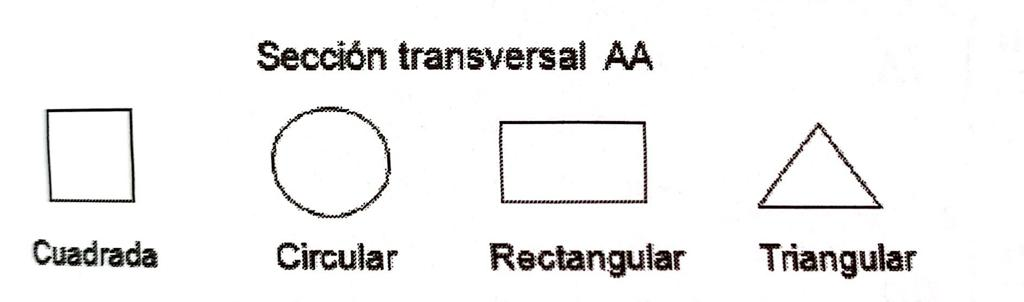
\includegraphics[width=8cm]{ttub.jpeg}
\caption{Tipos comunes de secciones transversales de tuberias (tomado de \cite{agudelo2011mecanica}).}
\label{ttub}
\end{figure}

Si se tiene un tanque grande del cual se conecta en la parte baja una tuberia (ver figura~\ref{cali}), los esfuerzos viscosos empiezan a crecer una vez el fluido ingresa a la tuber\'ia y por tanto la capa limite ($\delta$) tambien empieza a crecer a lo largo de la tuber\'ia. La zona inicial es una zona de flujo ideal en donde los esfuerzos viscosos son despreciales y por lo tanto la velocidades son uniformes. Una vez, el flujo sale de zona inicial, la capa limite crece en una zona de \emph{flujo no establecido} en donde se desarrollan los esfuerzos de corte. Es posible que cuando la entrada a la tuberia no se hace a trave\'es de una transision suave, se presente separacion del flujo de las paredes de la tuber\'ia generandose remolinos que viajan y desaparecen a lo largo de la zona de flujo no establecido generandoe \emph{presiones negativas} a velocidades muy altas. Una vez las capas limites alderdor y crecientes en direccion del flujo se encuentran es cuando se tiene un \emph{flujo establecido} o flujo real gobernado por los esfuerzos de corte con una districi\'on no uniforme de velocidades.
  

\begin{figure}[h]
\centering
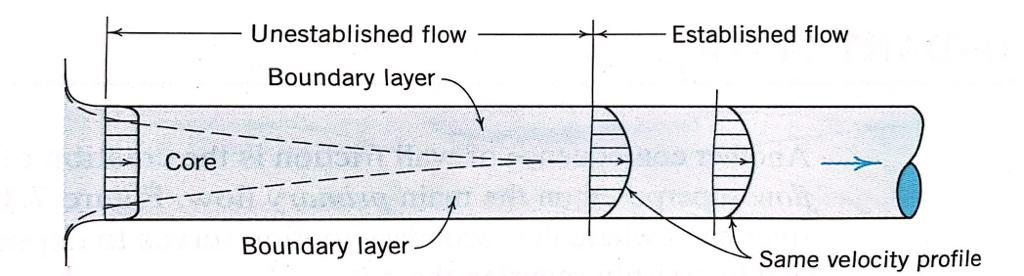
\includegraphics[width=8cm]{cali.jpeg}
\caption{Desarrollo de la capa limite a lo largo de una tuber\'ia (tomado de \cite{street471elementary}).}
\label{cali}
\end{figure}

El mecanismo de crecimiento de la capa limite se puede describir como sigue. Cuando el fluido entra a la tuber\'ia se desarrollan altos valores de $dv/dy$, donde $y$ es la direccion vertical. Estos altos gradientes ocurren dentro de la capa limite y son debido a los esfuerzos debido a la fricci\'on los cuales tratan de frenar el flujo. Dicha capa crece en la direccion del flujo hasta el punto en el que se encuentran. A partir de este punto de encuentro la friccion de fuerzas de friccion influencian el flujo y es toda secci\'on rotacional.

El flujo dentro de la capa limite puede ser laminar o turbulento. Si el numero de Reynolds $Re = \frac{Vd}{\nu}$, donde $V$ es la velocidad media del flujo, $d$ es el di\'ametro de la tuberia y $\nu$ es la viscosidad cinem\'atica, es $Re < 2100$, se puede inferir que el \emph{flujo laminar establecido} resulta del crecimiento de la capa limite laminar. En este caso la longitud que toma el establecimiento de este flujo es $\frac{x}{d} \approx \frac{Re}{20}$. Si el $Re$ aumenta levemente el flujo sera laminar a lo largo de $\frac{x}{d} \approx \frac{Re}{20}$ y luego sera transisional antes de que el flujo este establecido. Si $Re >> 2100$ la capa limite sera turbulenta. Para $Re$ altos, en casos practicos se puede decir que la longitud $x$ de la zona de flujo puede ser hasta $x \approx 100 d$. Sin embargo el flujo es establecido para valores mayores a $\frac{x}{d} \approx 20$. De acuerdo con esto, es posible notar que la energia en un flujo establecido disminuye a lo largo de la tuberia. Note que la energia debido a la cabeza de presi\'on disminuye a lo largo de la tuber\'ia debido a los esfuerzos de corte generados por la friccion dendro del flujo establecido. 
  
\begin{figure}[h]
\centering
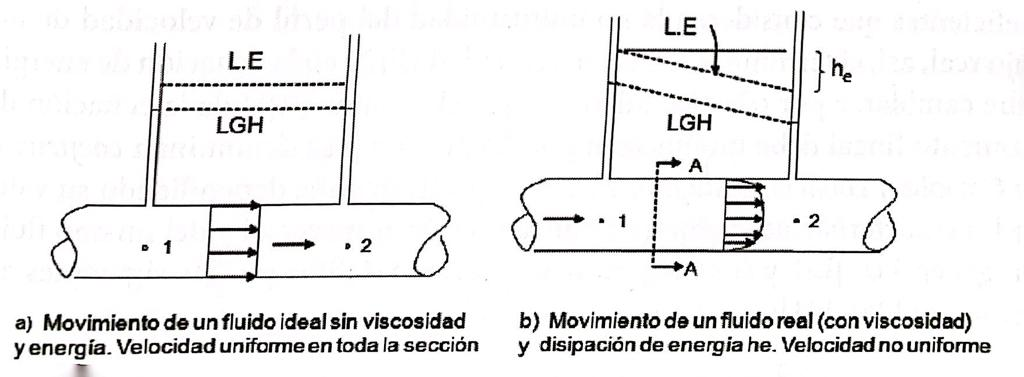
\includegraphics[width=8cm]{fifr.jpeg}
\caption{Linea de gradiente hidra\'aulico (LGH) y de energia (LE) en un a) fluido ideal y en un b) fluido real (tomado de \cite{agudelo2011mecanica}).}
\label{fifr}
\end{figure}

%%%%%%%%
\section{Esfuerzo de corte y perdidas de cabeza de energ\'ia}
Los esfuerzos de corte son producidos debido a la turbulencia del flujo o la viscosidad del fluido lo que con lleva a una resistencia al flujo que se traduce en perdidas de energ\'ia. Una pregunta clave, que se derivaria es ¿Cuales son los efectos de las fuerzas de fricci\'on sobre la superficie de un volumen de control, por ejemplo,  en una tuber\'ia?. Para esto analizaremos los esfuerzos de corte ($\tau$) en un  flujo 1D compresible y permanente a trav\'es de la tuber\'ia inclinada de la figura~\ref{tau}.
   
\begin{figure}[h]
\centering
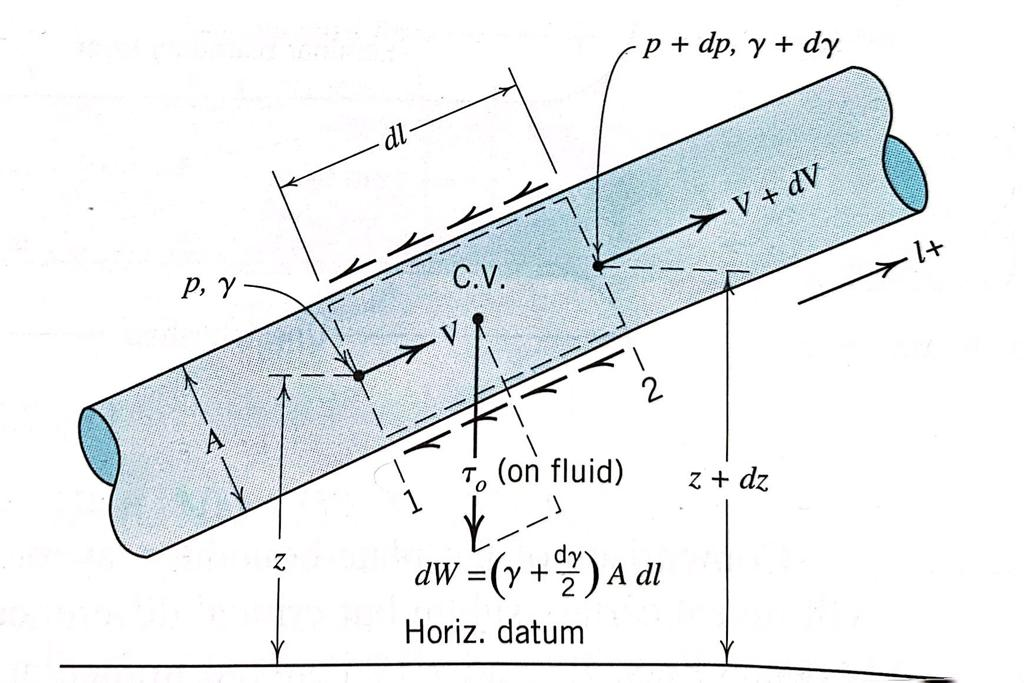
\includegraphics[width=8cm]{tau.jpeg}
\caption{Fuerzas actuantes sobre el volumen de control en la tuber\'ia inclinada (tomado de \cite{street471elementary}).}
\label{tau}
\end{figure}

Aplicando la \emph{ecuaci\'on de conservaci\'on de candidad de movimiento lineal} para las fuerzas actuantes en la direcci\'on del flujo sobre el volumen de control entre las secciones 1 y 2 en la  figura~\ref{tau}, tenemos que las fuerzas fundamentales que actuan son las \emph{fuerzas de presi\'on}, las \emph{fuerzas gravitacionales} y las \emph{fuerzas viscosas}. Por esto se tiene:

\begin{equation}
pA - (p+dp)A - \tau_{o} P dl - \left( \gamma + \frac{d \gamma}{2} \right)A dl \frac{dz}{dl} = (V+dV)^2 A (\rho +d \rho)- V^2 A \rho
\label{tau1}
\end{equation}

donde $V$ es la velocida del flujo, $p$ es la presi\'on en la secci\'on, $P$ es el perimetro de la secci\'on, $A$ es el area de la secci\'on transversal, $\tau_{o}$ es el esfuerzo de corte en la superficie de control, $dl$ es la longitud del volumen de control, $dV$ es un cambio en la velocidad a trav\'es de $dl$, $dz$ es la diferencia de alturas entre las secciones 1 y 2, $\rho$ es la densidad del fluido, $\gamma$ es el peso espec\'ifico del fluido, $d \rho$ es un cambio de $\rho$ a trav\'es de $dl$ y $d \gamma$ es el cambio del peso espec\'ifico a lo largo de $dl$. Note que $\left( \gamma + \frac{d \gamma}{2} \right) A dl \frac{dz}{dl} = dW \frac{dz}{dl}$, donde $dW \frac{dz}{dl}$ es el peso del fluido en el volumen de control en la direcci\'on contraria del flujo, donde $\frac{dz}{dl}=\sin \theta$ y $\theta$ es el angulo de inclinaci\'on de la tuber\'ia. Teniendo en cuenta que entre 1 y 2 los efectos de turbinas y bombas son despreciables, dividiendo por $A\gamma$, donde $\gamma = \rho g$ y despreciando los terminos que contengan productos de diferenciales,  la ecuaci\'on~\ref{tau1} queda: 
 
\begin{equation}
\frac{dp}{\gamma} + d\left( \frac{V^2}{2g} \right) + dz = -\frac{\tau_{o} dl}{\gamma R_h}
\label{tau2}
\end{equation}

donde $R_h = \frac{A}{P}$ es el radio hidr\'aulico de la secci\'on. Para \emph{flujo incompresible} en la tuber\'ia de la figura~\ref{tau}  y suponiendo que la tuberia es de secci\'on constante, significa que $\tau_{o}$ no es funcion de $l$ y que $\gamma$ es constante por lo que $d\left( \frac{1}{\gamma} \right)=0$. Por lo tanto la ecuaci\'on~\ref{tau2} queda:

\begin{equation}
d \left( \frac{p}{\gamma} +\frac{V^2}{2g} + z \right) = -\frac{\tau_o dl}{\gamma R_h}
\label{tau3}
\end{equation}

Integrando la ecuaci\'on~\ref{tau3} entre las secciones 1 y 2, queda: 

\begin{equation}
\left( \frac{p_1}{\gamma} +\frac{V_1^2}{2g} + z_1 \right) - \left( \frac{p_2}{\gamma} +\frac{V_2^2}{2g} + z_2 \right) = \frac{\tau_o (l_2 - l_1 )}{\gamma R_h}  
\label{tau4}
\end{equation}

Note que la diferencia de energ\'ia entre las secciones 1 y 2 (termino izquierdo de la ecuaci\'on~\ref{tau4}) es la caida de energ\'ia entre las dos secciones, por lo que la ecuaci\'on~\ref{tau4} se expresa como:

\begin{equation}
\left( \frac{p_1}{\gamma} +\frac{V_1^2}{2g} + z_1 \right) - \left( \frac{p_2}{\gamma} +\frac{V_2^2}{2g} + z_2 \right) = \Delta (EL) = h_{L_{1-2}}
\label{tau5}
\end{equation}

donde $\Delta (LE)$ es la caida de la l\'inea de energ\'ia o la perdida de energ\'ia entre 1 y 2 ($h_{L_{1-2}}$). Las perdidas de energ\'ia se pueden expresar como:

\begin{equation}
\color{red}\boxed{\color{black} h_{L_{1-2}} = \frac{\tau_o (l_2 - l_1 )}{\gamma R_h} }  
\label{tau6}
\end{equation}

Note que en la ecuaci\'on~\ref{tau6} quiere decir que las perdidas de energia en el volumen de control son directamente proporcionales a la longitud del volumen de control ya los esfuerzos cortantes ejercidos por las paredes de la tuber\'ia sobre las paredes del volumen de control. Las perdidas de energ\'ia son ademas inversamente proporcionales al radio hidr\'aulico del volumen de control. Si la tuberia es de secci\'on circular de radio $R$, $R_h = \frac{\pi r^2}{2\pi r} = \frac{r}{2}$,  la ecuaci\'on~\ref{tau6} quedar\'ia:

\begin{equation}
\color{red}\boxed{\color{black} h_{L_{1-2}} = \frac{2\tau_o (l_2 - l_1 )}{\gamma r} } 
\label{tau7}
\end{equation}

En terminos generales,  $\tau$ se puede expresar a parti de la ecuaci\'on~\ref{tau7}:
 
\begin{equation}
\color{red}\boxed{\color{black} \tau = \left( \frac{\gamma h_L }{2l} \right)r }
\label{tau8}
\end{equation}

donde $r$ es una distancia radial y $l$ es la longitud de la tuber\'ia. Note que $\tau$ varia linealmente con $r$ (ver figura~\ref{taun}) donde le $\tau_{max} = \tau_o$ se logra cuando $r=R$ (paredes de la tuber\'ia). Note que las ecuaciones anteriores fueron deducidas independiente si el flujo es laminar o turbulento.  

\begin{figure}[h]
\centering
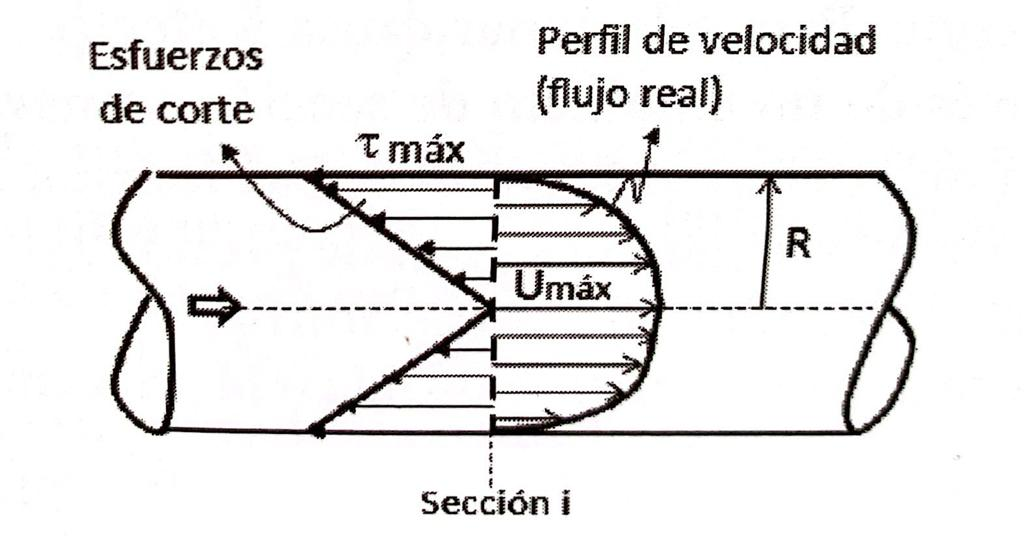
\includegraphics[width=8cm]{taun.jpeg}
\caption{Perfil de velocidades y esfuerzos de corte (tomado de \cite{agudelo2011mecanica}).}
\label{taun}
\end{figure}


% Ej 7.6 Street and Vennard
\begin{shaded}
\begin{exa}
Agua fluye en un conducto rectangular de secci\'on 0.9 m de ancho por 0.6 m de alto. La perdida de cabeza de energ\'ia en este conducto de 60 m de longitud fue determinada experimentalmente e igual 10 m. a) Cacular el esfuerzo de corte en las paredes del conducto. Si el conducto es de secci\'on circular de diametro $D = 0.6$m, b) ¿cual es el esfuerzo cortante en las paredes? y c) ¿dentro del flujo en un punto a 200 mm de las paredes?
\end{exa}
\end{shaded}

%%%%%%%%
\section{Experimentos de Reynolds}
Osborne Reynolds en 1883 mediante un experimento el cual consistio en establecer un flujo de agua a trav\'es de una tuber\'ia de vidrio en el que la velocidad era controlada por una valvula a la salida de la tuberia (ver figura~\ref{reyn}). A la entrada de la tube\'ia se inyecta una tinta que tiene un peso espec\'ifico igual al del agua. Reynolds encontr\'o que cuando la valvula esta ligeramente abierta, las particulas de tinta se mueven de forma ordenada formando un filamento y a manera de capas que se deslizan una sobre otra sin mezclarse. Sin embargo, a medida que la valvula se va abriendo, se alcanza una condicion en la cual la tinta presenta un movimiento fluctuante a medida que avanza en la tuber\'ia, en donde las particulas de la tinta se mueven caoticamente mezclandose. Al primer tipo de flujo se le llamo \emph{laminar} y al segundo \emph{turbulento}.

% FIg 9.2 from Shames 
\begin{figure}[h]
\centering
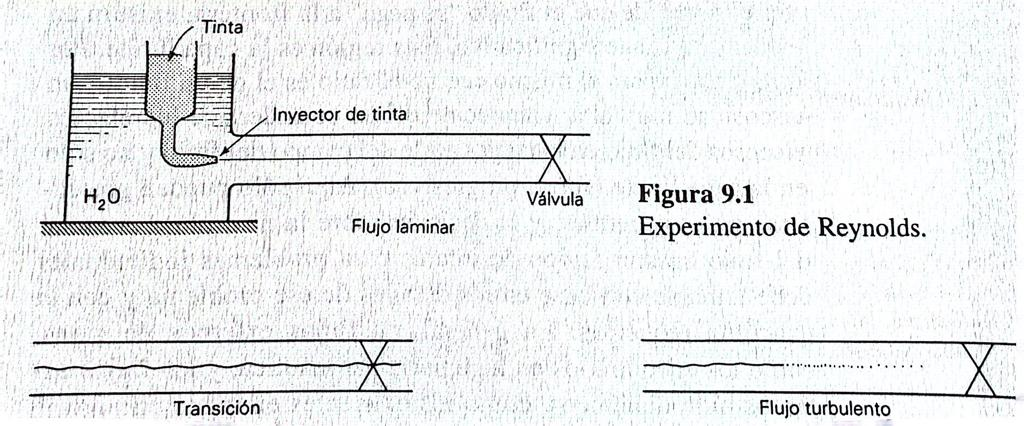
\includegraphics[width=8cm]{reyn.jpeg}
\caption{Experimento de Reynolds (tomado de \cite{irving2010fluid}).}
\label{reyn}
\end{figure}

% FIg 9.4 y 9.5 from Shames 
\begin{figure}[h]
\centering
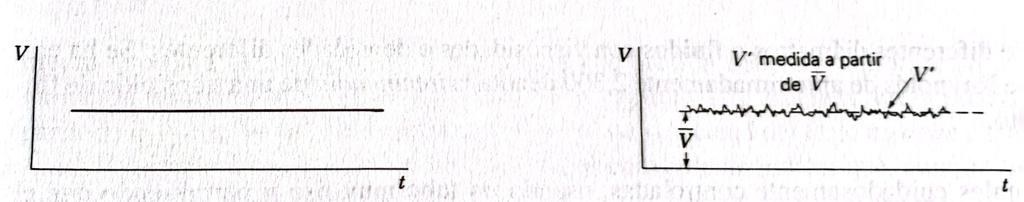
\includegraphics[width=8cm]{reyn1.jpeg}
\caption{Velocidad para flujo laminar y flujo turbulento (tomado de \cite{irving2010fluid}).}
\label{reyn1}
\end{figure}

Reynolds encontro que el comportamiento de flujo se podia correlacionar con un parametro adimensional que relacionaba las fuerzas de inercia y las fuerzas viscosas, el cual es conocido como el \emph{numero de Reynolds (Re)}:

\begin{equation}
\color{red}\boxed{\color{black} Re = \frac{VD}{\nu} = \frac{1.273Q}{\nu D} }
\label{rey}
\end{equation}

donde $D$ es el diametro de la tuber\'ia. 

Reynolds encontro que flujo laminar se obtenia para valores de $Re<12000$, mientras que el flujo turbulento se lograba con $Re>50000$. Sin embargo estos valores encontrados por Reynolds se obtuvieron para condiciones alejadas de lo que es un sistema de conducci\'on real y que ocurren comunmente en ingenier\'ia. Para propositos practicos en tuber\'ias comerciales se ha encontrado que:
$$
Re < 2000 \rightarrow \text{flujo laminar}
$$
$$
2000 < Re < 4000 \rightarrow \text{flujo de transici\'on}
$$
$$
Re > 4000 \rightarrow \text{flujo de turbulento}
$$ 

%%%%%%%%
\section{Flujo laminar}


% REFERENCES
\bibliographystyle{plain} % We choose the "plain" reference style
\bibliography{refs} % Entries are in the refs.bib file



\end{document}
